\documentclass[ucs,10pt]{beamer}
 
% Template for talks using the Logo of STCE and Corporate Design of RWTH Aachen
% adapted from:
% https://www.mi.fu-berlin.de/w/Mi/BeamerTemplateCorporateDesign

\usepackage{amsmath,dsfont,listings}
% ** for picture **
\usepackage{graphicx}

%%% STCE logo
% small version for upper right corner of normal pages
\pgfdeclareimage[height=0.9cm]{university-logo}{rwth_i12_softw-werkz_en_rgb.png}
\logo{\pgfuseimage{university-logo}}
% large version for upper right corner of title page
\pgfdeclareimage[height=1cm]{big-university-logo}{rwth_i12_softw-werkz_en_rgb.png}
\newcommand{\titleimage}[1]{\pgfdeclareimage[height=2cm]{title-image}{#1}}
\titlegraphic{\pgfuseimage{title-image}}
%%% end STCE logo

% NOTE: 1cm = 0.393 in = 28.346 pt;    1 pt = 1/72 in = 0.0352 cm
\setbeamersize{text margin right=3.5mm, text margin left=7.5mm}  % text margin

% colors to be used
\definecolor{text-grey}{RGB}{51, 51, 51} % grey text on white background
\definecolor{bg-grey}{rgb}{0.66, 0.65, 0.60} % grey background (for white text)
\definecolor{rwth-blue}{RGB}{0, 83, 159} % blue text
\definecolor{rwth-green}{RGB}{153, 204, 0} % green text
\definecolor{rwth-red}{RGB}{204, 0, 0} % red text (used by \alert)

% switch off the sidebars
% TODO: loading \useoutertheme{sidebar} (which is maybe wanted) also inserts
%   a sidebar on title page (unwanted), also indents the page title (unwanted?),
%   and duplicates the navigation symbols (unwanted)
\setbeamersize{sidebar width left=0cm, sidebar width right=0mm}
\setbeamertemplate{sidebar right}{}
\setbeamertemplate{sidebar left}{}
%    XOR
% \useoutertheme{sidebar}

% frame title
% is truncated before logo and splits on two lines
% if neccessary (or manually using \\)
\setbeamertemplate{frametitle}{%
    \vskip-30pt \color{purple}\large%
    \begin{minipage}[b][23pt]{80.5mm}%
    \flushleft\insertframetitle%
    \end{minipage}%
}

%%% title page
% TODO: get rid of the navigation symbols on the title page.
%   actually, \frame[plain] *should* remove them...
\setbeamertemplate{title page}{
% upper right: STCE logo
\vskip2pt\hfill\pgfuseimage{big-university-logo} \\
\vskip6pt\hskip3pt
% title image of the presentation
% set the title and the author
\begin{center}
\vskip4pt
\large \inserttitle \vskip5pt  \small \insertsubtitle
\vskip8pt
	\normalsize \insertauthor %\\ 
	%\includegraphics[width=2cm]{../../foto_naumann}	
\\ [5mm]
	\footnotesize \insertinstitute 
\end{center}
}
%%% end title page

%%% colors
\usecolortheme{lily}
\setbeamercolor*{normal text}{fg=black,bg=white}
\setbeamercolor*{alerted text}{fg=rwth-red}
\setbeamercolor*{example text}{fg=rwth-green}
\setbeamercolor*{structure}{fg=rwth-blue}

\setbeamercolor*{block title}{fg=white,bg=black!50}
\setbeamercolor*{block title alerted}{fg=white,bg=black!50}
\setbeamercolor*{block title example}{fg=white,bg=black!50}

\setbeamercolor*{block body}{bg=black!10}
\setbeamercolor*{block body alerted}{bg=black!10}
\setbeamercolor*{block body example}{bg=black!10}

\setbeamercolor{bibliography entry author}{fg=rwth-blue}
% TODO: this doesn't work at all:
\setbeamercolor{bibliography entry journal}{fg=text-grey}

\setbeamercolor{item}{fg=rwth-blue}
\setbeamercolor{navigation symbols}{fg=text-grey,bg=bg-grey}
%%% end colors

%%% headline
\setbeamertemplate{headline}{
\vskip4pt\hfill\insertlogo\hspace{3.5mm} % logo on the right

\vskip6pt\color{rwth-blue}\rule{\textwidth}{0.4pt} % horizontal line
}
%%% end headline

%%% footline
\newcommand{\footlinetext}{\insertshortinstitute, \insertshorttitle}
\setbeamertemplate{footline}{
\vskip5pt\color{rwth-blue}\rule{\textwidth}{0.4pt}\\ % horizontal line
\vskip2pt
\makebox[123mm]{\hspace{7.5mm}
\color{rwth-blue}\footlinetext
\hfill \raisebox{-1pt}{\usebeamertemplate***{navigation symbols}}
\hfill \insertframenumber}
\vskip4pt
}
%%% end footline

%%% settings for listings package
\lstset{extendedchars=true, showstringspaces=false, basicstyle=\footnotesize\sffamily, tabsize=2, breaklines=true, breakindent=10pt, frame=l, columns=fullflexible}
\lstset{language=C++} % this sets the syntax highlighting
\lstset{mathescape=true} % this switches on $...$ substitution in code
% enables UTF-8 in source code:
\lstset{literate={ä}{{\"a}}1 {ö}{{\"o}}1 {ü}{{\"u}}1 {Ä}{{\"A}}1 {Ö}{{\"O}}1 {Ü}{{\"U}}1 {ß}{\ss}1}
%%% end listings
  

\begin{document}
\title[{\tt info@stce.rwth-aachen.de}]{\textcolor{rwth-blue}{Software Lab Computational Engineering Science} \vspace{.2cm} \\ {\small Group 12, Exception Handling}}
\author[Group 12)]{Aaron Floerke, Arseniy Kholod, Xinyang Song and Yanliang Zhu} 
\institute[Software Lab CES]{
{Informatik 12: Software and Tools for Computational Engineering (STCE)} \\ RWTH Aachen University \vspace{.5cm}
}
\date[]{24.06.2024}

\begin{frame}[plain]
\titlepage
\end{frame}

\begin{frame}
	\frametitle{Contents}
\tableofcontents
\end{frame}

\section{Analysis}

\subsection{User Requirements}

\begin{frame}
\frametitle{Analysis \\
	\small \color{rwth-blue} User Requirements}
	\begin{itemize}
		\item Extend cppNum v2.4 and v2.5 with appropriate C++ exception handling.
		\item Desing at least three scalable sufficiently distinct case studies.
		\item Compare general behavior and run times with the exception handling-free version.
	\end{itemize}
\end{frame}

\begin{frame}
\frametitle{Analysis \\
	\small \color{rwth-blue} Definition Exception Handling}
	\begin{itemize}
		\item Exception handling is a programming concept used to manage errors and unusual conditions that arise during program execution. It allows for controlled responses to errors, ensuring the program can handle them gracefully without crashing. Key components include try, catch (or except), and finally blocks. (ChatGPT)
	\end{itemize}
\end{frame}

\subsection{System Requirements}

\begin{frame}
\frametitle{Analysis \\
	\small \color{rwth-blue} System Requirements}
	Functional:
	\begin{itemize}
		\item \textbf{Exception Handling:}
		\begin{itemize}
			\item An exception is thrown, if unintended input is put into the system
			\item An exception is thrown when the system behaves in an unintended way. 
                	\item An exception should be handled in such a way, as to prevent a potential crash of the system, if possible.
			\item The system must handle also exceptions from third-party libraries.
			\item The system must integrate C++ exception handling mechanisms in cppNum versions v2.4 and v2.5.
			\item The system must log all exceptions with appropriate error messages.
        	        \item A thrown exception should enhance the users ability to find bugs.
		\end{itemize}
		\item \textbf{Case Studies:}
		\begin{itemize}
			\item The system must implement at least three scalable and distinct case studies to test the modified cppNum library.
			\item Each case study must include a specific scenario that can trigger exceptions.
		\end{itemize}
		\item \textbf{Performance Comparison:}
		\begin{itemize}
			\item The system must compare the general behavior and run times of the modified cppNum versions with the original exception-free versions.
			\item The comparison results must be documented and include detailed performance metrics.
		\end{itemize}
	\end{itemize}
\end{frame}

\begin{frame}
\frametitle{Analysis \\
	\small \color{rwth-blue} System Requirements}
	Nonfunctional:
	\begin{itemize}
		\item \textbf{Exception Structure:}
		\begin{itemize}
			\item An exception is a class object.
			\item All cppNum exception classes have a single parent class to provide a clear structure.
			\item All exception classes are inherited from std::exception to catch together with other exceptions, potentially generated by third-party libraries.
		\end{itemize}
		\item \textbf{Exception Logic:}
		\begin{itemize}
			\item  The system provides stack trace. Each cppNum function that catches an exception indicates it and rethrows it up the call tree. The final function displays the exception message.  
		\end{itemize}
		\item \textbf{Performance:}
		\begin{itemize}
			\item The system must ensure that the overhead introduced by exception handling is minimized.
			\item The system should not degrade the performance of cppNum versions v2.4 and v2.5.
		\end{itemize}
        \end{itemize}
\end{frame}

\begin{frame}
\frametitle{Analysis \\
	\small \color{rwth-blue} System Requirements}
	\begin{itemize}	
		\item \textbf{Reliability:}
                \begin{itemize}
                        \item The system must handle exceptions gracefully to prevent crashes and ensure smooth operation.
                        \item The system must be able to recover from exceptions and continue processing if possible.
                \end{itemize}
        	\item \textbf{Usability:}
		\begin{itemize}
			\item The system must provide clear and informative error messages to users when exceptions occur.
			\item The system should document the scenarios under which exceptions are raised and how they are handled.
		\end{itemize}
		\item \textbf{Maintainability:}
		\begin{itemize}
			\item The code implementing exception handling must be well-documented and follow coding standards.
			\item The system must use modular and clean code to facilitate future updates and maintenance.
		\end{itemize}
		\item \textbf{Scalability:}
		\begin{itemize}
			\item The system must be able to handle large datasets and complex computations in the case studies without significant performance degradation.
			\item The system must be designed to easily incorporate future case studies.
		\end{itemize}
	\end{itemize}
\end{frame}

\begin{frame}
\frametitle{Design \\
	\small \color{rwth-blue} Principal Components and Third-Party Software}
	\begin{itemize}
		\item Exceptions from third-party libraries.
		\begin{itemize}
			\item Third-Party libraries: Eigen and AD.
			\item Eigen and AD can throw exceptions inherited from std::exception.
			\item Wrap each connection point to Eigen and AD with a try-catch block to handle possible exceptions.
			\item Stack Trace: Every cppNum function that catches an exception indicates its occurrence and rethrows it to the next function in the recursive call tree. The final function prints the exception message and returns without crashing.
		\end{itemize}
		\item cppNum exceptions
		\begin{itemize}
			\item Implement cppNum exception classes inherited from std::exception to manage exceptions generated by cppNum itself.
			\item Implement checks for the applicability of LU and LLT decompositions using functions from Eigen. Generate custom cppNum exceptions for error cases.
		\end{itemize}
		\item The user does not handle exceptions directly as they are caught within cppNum. Instead, the user receives a stack trace and an explanatory string as terminal output.
	\end{itemize}
\end{frame}

\subsection{Class Model}

\begin{frame}
\frametitle{Design \\
	\small \color{rwth-blue} Class Model: cppNum exceptions}
	\begin{figure}
                \centering
                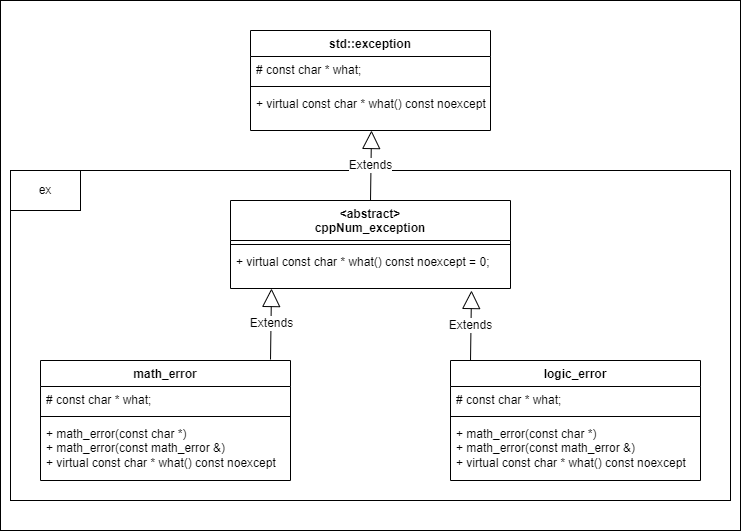
\includegraphics[width=0.8\textwidth]{figures/class_diagramm.png}
        \end{figure}
\end{frame}


\section{Implementation}

\subsection{Development Infrastructure}

\begin{frame}
\frametitle{Implementation \\
	\small \color{rwth-blue} Development Infrastructure}
	\begin{itemize}	
		\item \textbf{1. Operating System:}
			\begin{itemize}
				\item Xubuntu
			\end{itemize}
		\item \textbf{2. Programming Language and Compiler:}
			\begin{itemize}
				\item Programming Language: C++.
				\item Compiler: GCC.
			\end{itemize}
		\item \textbf{3. Libraries:}
			\begin{itemize}
				\item Eigen: A C++ library for linear algebra, providing efficient matrix and vector operations.
				\item AD: Provide a complete C++ solution for implementing algorithmic differentiation in numerical computations.
			\end{itemize}
		\item \textbf{4. Version Control System:}
			\begin{itemize}
				\item GitHub: Remote code repositories for team collaboration, code reviews, and version control. \url{https://github.com/ArseniyKholod/stce_ss24_ex12}
			\end{itemize}
		\item \textbf{5. Frameworks:}
			\begin{itemize}
				\item Doxygen: Used for generating project documentation, helping the team understand and maintain the code better.
				\item Makefile: For build management.
			\end{itemize}
	\end{itemize}
\end{frame}



\subsection{Source Code}

\begin{frame}
\frametitle{Implementation \\
	\small \color{rwth-blue} Sutructure of source code}
	\begin{columns}
         	\begin{column}{0.5\textwidth}
			\setlength{\parindent}{2em}
			cppNum \textbf{v2.4} \newline
			  \indent exceptions \newline
		    	    \indent \indent cppNum\_exception.hpp \newline
		   	    \indent \indent math\_error.hpp \newline
		    	    \indent \indent logic\_error.hpp \newline
		  	  \indent convexObjective \newline
		    	    \indent \indent objective.hpp \newline
		    	    \indent \indent newton.hpp \newline
		    	    \indent \indent minimizer.hpp \newline
		  	  \indent algebraicSystem \newline
		    	    \indent \indent system.hpp \newline
		    	    \indent \indent solver.hpp \newline
		    	    \indent \indent newton.hpp \newline
		  	  \indent linearAlgebra.hpp \newline
		  	  \indent iteration.hpp \newline
		  	  \indent derivative.hpp \newline
		  	  \indent approximation.hpp \newline
		\end{column}
		\begin{column}{0.5\textwidth}
			\setlength{\parindent}{2em} \vspace{1mm} \newline
                	cppNum \textbf{v2.5} \newline
                  	  \indent exceptions \newline
                   	    \indent \indent cppNum\_exception.hpp \newline
               		    \indent \indent math\_error.hpp \newline
                	    \indent \indent logic\_error.hpp \newline
                	  \indent differentialSystem \newline
               		    \indent \indent system.hpp \newline
                 	    \indent \indent integrator.hpp \newline
                 	    \indent \indent implicitEuler.hpp \newline
                 	  \indent algebraicSystem \newline
                 	    \indent \indent system.hpp \newline
                 	    \indent \indent solver.hpp \newline
                  	    \indent \indent newton.hpp \newline
                 	  \indent linearAlgebra.hpp \newline
               	 	  \indent iteration.hpp \newline
                 	  \indent derivative.hpp \newline
                 	  \indent approximation.hpp \newline
		 	  \indent evolution.hpp \newline
     		\end{column}
	\end{columns}
\end{frame}

\begin{frame}[fragile]
\frametitle{Source Code \\
        \small \color{rwth-blue} cppNum/exceptions/cppNum\_exception.hpp v2.4 and v2.5 }
	\textbf{Important}: The following slides do not show all changes introduced to v2.4 and v2.5; they cover only essential changes. Sometimes changes had to be made multiple times, and only one instance is shown here. Code that remains unchanged is represented as \textbf{...} to save space on the slides. If you are interested in seeing all the changes introduced by our group, please refer to  \url{https://github.com/ArseniyKholod/stce_ss24_ex12/tree/main/ex12}. 
	\begin{lstlisting}
	#pragma once
	#include <exception>
	namespace ex{
  	  /// Abstract basic class for all cppNum exceptions
  	  class cppNum_exception: public std::exception{
    	    public:
    	      virtual const char* what() const noexcept =0;
  	  };
	}
	\end{lstlisting}
\end{frame}

\begin{frame}[fragile]
\frametitle{Source Code \\
        \small \color{rwth-blue} cppNum/exceptions/math\_error.hpp v2.4 and v2.5 }
	\begin{lstlisting}
        #pragma once
        #include "cppNum_exception.hpp"
        #include <string>
        namespace ex{
          /// An exception class to handle mathematical errors
          class math_error: public cppNum_exception {
            protected:
              /// Error message
              const char* what_arg;
            public:
              /// Constructor to initialize error message
              math_error(const char*);
              /// Copy constructor
              math_error(const math_error&);
              /// Returns explanatory string
              virtual const char* what() const noexcept{
                return what_arg;
              }
          };

          math_error::math_error(const char* what_arg) : what_arg(what_arg){}
          math_error::math_error(const math_error& err){
            what_arg = err.what_arg;
          }
        }
        \end{lstlisting}
\end{frame}

\begin{frame}[fragile]
\frametitle{Source Code \\
        \small \color{rwth-blue} cppNum/exceptions/logic\_error.hpp v2.4 and v2.5 }
	\begin{lstlisting}
	#pragma once
	#include "cppNum_exception.hpp"
	#include <string>
	
	namespace ex{
	  /// An exception class to handle logical errors
	  class logic_error: public cppNum_exception {
	    protected:
	      /// Error message
	      const char* what_arg;
	    public:
	      /// Constructor to initialize error message
	      logic_error(const char*);
	      /// Copy constructor
	      logic_error(const logic_error&);
	      /// Returns explanatory string
	      virtual const char* what() const noexcept{
	        return what_arg;
	      }
	  };
		
	  logic_error::logic_error(const char* what_arg) : what_arg(what_arg){}
	  logic_error::logic_error(const logic_error& err){
	    what_arg = err.what_arg;
	  }
	}
	\end{lstlisting}
\end{frame}

\begin{frame}[fragile]
\frametitle{Source Code \\
        \small \color{rwth-blue} cppNum/linearAlgebra.hpp v2.4 and v2.5, LU }
	\begin{lstlisting}
	...
	template<typename T>
	struct lu_solver_t {
	  static la::vector_t<T> run(const la::matrix_t<T>& A, const la::vector_t<T>& b) {
	    try{
	      //matrix have to be square
	      if(A.cols() != A.rows())
	        throw(ex::math_error("Matrix is not square, LU decomposition is not applicable"));
	      //matrix and vector must have equal number of rows
	      if(A.rows() != b.rows())
	        throw(ex::math_error("Matrix and rhs-vector have diffirent number of rows, linear system is not uniquely solvable"));
	      //matrix have to be invertible
	      if(A.determinant() == 0)
	        throw(ex::math_error("Matrix is singular, applying LU algorithm for solving a linear system is not possible."));
	      return A.lu().solve(b);
	    }
	    catch(...){
	      std::cerr<<"Exception was caught in la::lu_solver_t::run, throw it further."<<std::endl;
	      throw;
	    }
	  }
  	};
	...
	\end{lstlisting}
\end{frame}

\begin{frame}[fragile]
\frametitle{Source Code \\
        \small \color{rwth-blue} cppNum/linearAlgebra.hpp v2.4 and v2.5, LLT }
	\begin{lstlisting}
	  ...
	  template<typename T>
	  struct llt_solver_t {
	    static la::vector_t<T> run(const la::matrix_t<T>& A, const la::vector_t<T>& b) {
	      try{
	        //matrix have to be squared
	        if(A.cols() != A.rows())
	          throw(ex::math_error("Matrix is not square, LLT decomposition is not applicable"));
	        //matrix and vector must have equak number of rows
	        if(A.rows() != b.rows())
	          throw(ex::math_error("Matrix and rhs-vector have diffirent number of rows, linear system is not uniquely solvable"));
	        //matrix have to be invertible
	        if(A.determinant() == 0)
	          throw(ex::math_error("Matrix is singular, applying LLT algorithm for solving a linear system is not possible."));
	        //matrix have to be symmetric positive definite
	        if(A.llt().info())
	          throw(ex::math_error("Matrix is not symmetric positiv definite, LLT decomposition is not applicable."));
	        return A.llt().solve(b);
	      }
	      catch(...){
	        std::cerr<<"Exception was caught in la::llt_solver_t::run, throw it further."<<std::endl;
	        throw;
	      }
	    }
  	  };
	  ...
        \end{lstlisting}
\end{frame}

\begin{frame}[fragile]
\frametitle{Source Code \\
        \small \color{rwth-blue} cppNum/derivative.hpp v2.4 and v2.5 }
	The content of each member function of derivative\_t was wrapped in a try block and followed by a catch block. For example, dFdx was handled this way, for all other functions exactly in the same way.
        \begin{lstlisting}
	...
	static la::matrix_t<T> dFdx(const la::vector_t<T>& x_v, const la::vector_t<T>& p_v) {
	  try{...
	  }
	  catch(...){
	    std::cerr<<"Exception was caught in derivative_t::dFdx, throw it further."<<std::endl;
	    throw;
	  }
	}
	...
        \end{lstlisting}
\end{frame}

\begin{frame}[fragile]
\frametitle{Source Code \\
        \small \color{rwth-blue} cppNum/algebraicSystem/newton.hpp v2.4 and v2.5 }
	\begin{lstlisting}
        ...
  	  template<typename T, typename SYSTEM_T, typename LINEAR_SOLVER_T>
	  la::vector_t<T> newton_solver_t<T,SYSTEM_T,LINEAR_SOLVER_T>::run(la::vector_t<T> x, const la::vector_t<T> &p) {
	    try{...
	    }
	    catch(...){
	      std::cerr<<"Exception was caught in as::newton_solver_t::run, throw it further."<<std::endl;
	      throw;
	    }
	  }
	...
        \end{lstlisting}
\end{frame}

\begin{frame}[fragile]
\frametitle{Source Code \\
        \small \color{rwth-blue} cppNum/convexObjective/newton.hpp v2.4 }
	The highest-level function in v2.4 is co::newton\_minimizer\_t::run. It handles exceptions by printing an explanatory message and returning an initial value to user without rethrowing the exception.
	\begin{lstlisting}[basicstyle=\tiny\sffamily]
	  ...
	  la::vector_t<AS_T> newton_minimizer_t<T,LINEAR_SOLVER_T>::F(const la::vector_t<AS_T> &x, const la::vector_t<AS_T>& p) {
	    try{
	      return derivative_t::dfdx<objective_t,AS_T>(x,p);
	    }
	    catch(...){
	      std::cerr<<"Exception was caught in co::newton_minimizer_t::F, throw it further."<<std::endl;
	      throw;
	    }
  	  }
	  ...
	  la::vector_t<T> newton_minimizer_t<T,LINEAR_SOLVER_T>::run(la::vector_t<T> x, const la::vector_t<T> &p) {
	    la::vector_t<T> x_initial(x);
	    try{
	      ...	
	      return x;
	    }
	    catch(const std::exception & e){
	      std::cerr<<"std:exception was caught in co::newton_minimizer_t::run with following message:"<<std::endl<<e.what()<<std::endl;
	    }
	    catch(...){
	      std::cerr<<"Exception of unknown type was caught in co::newton_minimizer_t::run."<<std::endl;
	    }
	    std::cerr<<"co::newton_minimizer_t::run returns an initial value of x. Check the correctness of the input."<<std::endl;
	    return x_initial;

	  }
	...
        \end{lstlisting}
\end{frame}

\begin{frame}[fragile]
\frametitle{Source Code \\
        \small \color{rwth-blue} cppNum/differentialSystem/implicitEuler.hpp v2.5 }
	The highest-level function in v2.5 is ds::implicitEuler\_integrator\_t::run. It handles exceptions by printing an explanatory message and returning an initial value to user without rethrowing the exception.
        \begin{lstlisting}
        ...
	  template<typename T>
	  la::vector_t<T> implicitEuler_integrator_t<T>::run(la::vector_t<T> x, const la::vector_t<T> &p) {
	    la::vector_t<T> x_initial(x);
	    try{...
	      return x;
	    }
	    catch(const std::exception & e){
	      std::cerr<<"std:exception was caught in ds::implicitEuler_integrator_t::run with following message:"<<std::endl<<e.what()<<std::endl;
	    }
	    catch(...){
	      std::cerr<<"Exception of unknown type was caught in ds::implicitEuler_integrator_t::run."<<std::endl;
	    }
	    std::cerr<<"ds::implicitEuler_integrator_t::run returns an initial value of x. Check the correctness of the input."<<std::endl;
	    return x_initial;
	  }
	...
        \end{lstlisting}
\end{frame}

\begin{frame}[fragile]
\frametitle{Source Code \\
        \small \color{rwth-blue} Additional: plot functions v2.4 and v2.5 }
	In all plot functions, we ensured that the requested state exists. These functions were wrapped in try-catch blocks. For example, in evolution\_t::plot from v2.5, and similarly for all other plots.
	\begin{lstlisting}
	template<typename T>
	void evolution_t<T>::plot(const std::string& filename, int i) const {
	  try{
	    std::ofstream ofs(filename);
	    assert(_states.size()==_times.size());
	    //check if requested state exists
	    if(i < 0 || i >= _states[0].rows())
	      throw(ex::logic_error("State outside range is requested."));
	    for (size_t k=0; k<_times.size(); ++k)
	      ofs << _times[k] << ' ' << _states[k](i) << std::endl;
	  }
	  catch(const std::exception & e){
	    std::cerr<<"std:exception was caught in evolution_t::plot with following message:"<<std::endl<<e.what()<<std::endl;
	  }
	  catch(...){
	    std::cerr<<"Exception of unknown type was caught in evolution_t::plot."<<std::endl;
	  }
	}
        \end{lstlisting}
\end{frame}

\section{Documentation}

\begin{frame}
\frametitle{Documentation \\
        \small \color{rwth-blue} Doxygen}
	Example is for v2.4, analogically for v2.5.
        \begin{figure}
		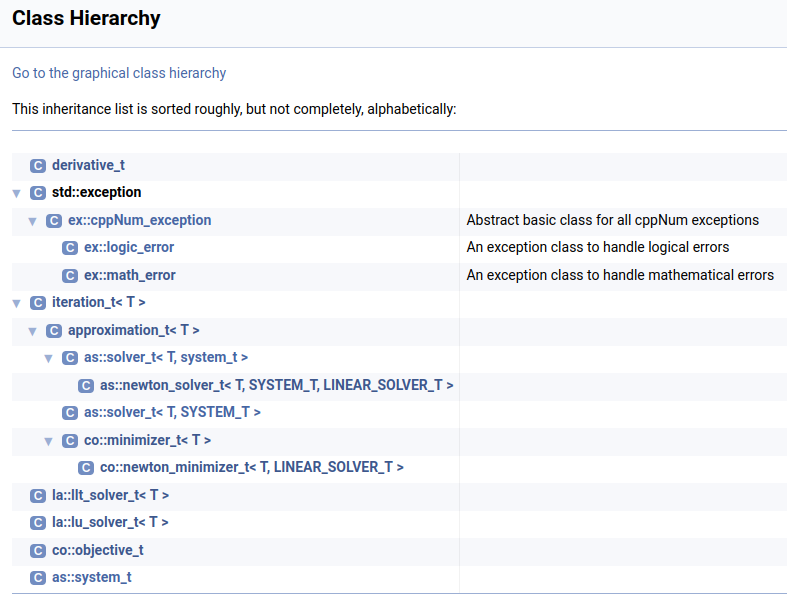
\includegraphics[width=0.65\textwidth]{figures/class_hierarchy_doc.png}                
        \end{figure}
\end{frame}

\begin{frame}
\frametitle{Documentation \\
        \small \color{rwth-blue} Doxygen}
	\begin{figure}[b]
		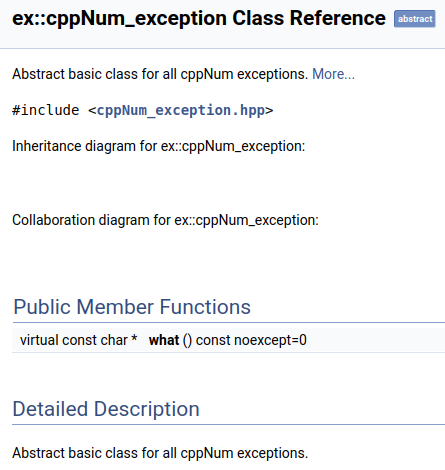
\includegraphics[width=0.35\textwidth]{figures/cppNum_exception_doc.png}
                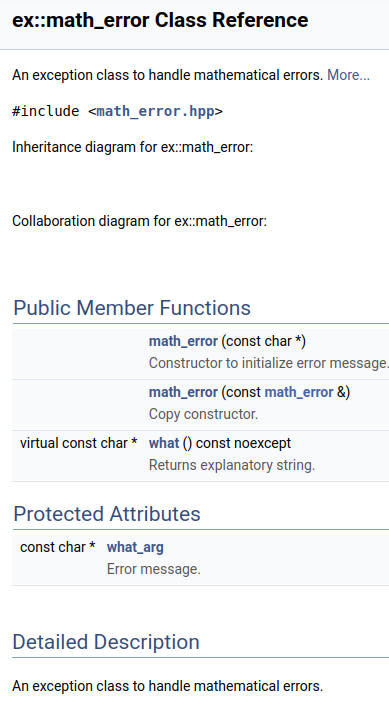
\includegraphics[width=0.3\textwidth]{figures/math_error_doc.png}
                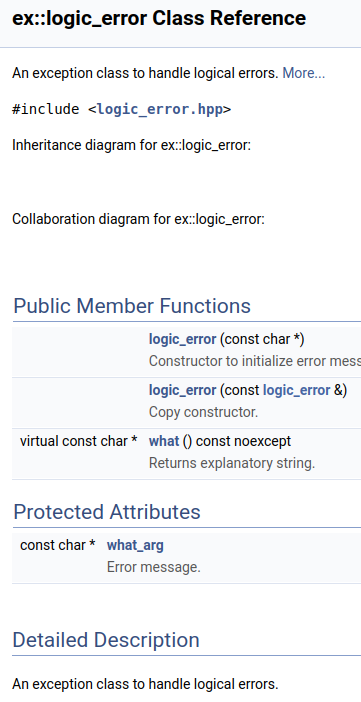
\includegraphics[width=0.28\textwidth]{figures/logic_error_doc.png}
        \end{figure}
\end{frame}

\section{Software Tests}

\begin{frame}[fragile]
\frametitle{Software Tests: Case Study for v2.4 \\
	\small \color{rwth-blue} Convex Objective: 4th order convex polynomial}
	The function is:
	$f(x, p) = \sum_{i=0}^{n-1} (0.5 \cdot (p(i) + x(i))^2 + 0.2 \cdot (x(i) - p(i))^4)$
	\begin{lstlisting}
		#pragma once
		#include "cppNum/convexObjective/objective.hpp"
		#include <cassert>
		#include <cmath>
		
		template<typename T> 
		T co::objective_t::f(const la::vector_t<T> &x, const la::vector_t<T> &p) { 
		using namespace std;
		int n=x.size(); assert(n>=1); assert(p.size()==n);
		T y=0;
		for (int i=0;i<n;++i) y+=0.5*pow(p(i)+x(i),2) + 0.2*pow(x(i)-p(i),4);
		return y;
		}
	\end{lstlisting}
	For time measurements:
	\begin{itemize}
		\item Initial value of x: $[-4, -4, ..., -4]$
		\item Parameters p: $[2, 2, ..., 2]$
	\end{itemize}
\end{frame}
	
\begin{frame}[fragile]
\frametitle{Software Tests: Case Study for v2.4 \\
	\small \color{rwth-blue} Convex Objective: cosh}
	The function is:
	$f(x, p) = \sum_{i=0}^{n-1} (\cosh(x(i) + p(i)))$
	\begin{lstlisting}
		#pragma once
		#include "cppNum/convexObjective/objective.hpp"
		#include <cassert>
		#include <cmath>
		
		template<typename T> 
		T co::objective_t::f(const la::vector_t<T> &x, const la::vector_t<T> &p) { 
		using namespace std;
		int n=x.size(); assert(n>=1); assert(p.size()==n);
		T y=0;
		for (int i=0;i<n;++i) y+=cosh(x(i)+p(i));
		return y;
		}
	\end{lstlisting}
        For time measurements:
        \begin{itemize}
                \item Initial value of x: $[-4, -4, ..., -4]$
                \item Parameters p: $[2, 2, ..., 2]$
        \end{itemize}
\end{frame}
	
\begin{frame}[fragile]
\frametitle{Software Tests: Case Study for v2.5 \\
	\small \color{rwth-blue} ODE: fountain chain}
	Investigate level of water in consecutive connected fountains.
	\begin{figure}
		\centering
		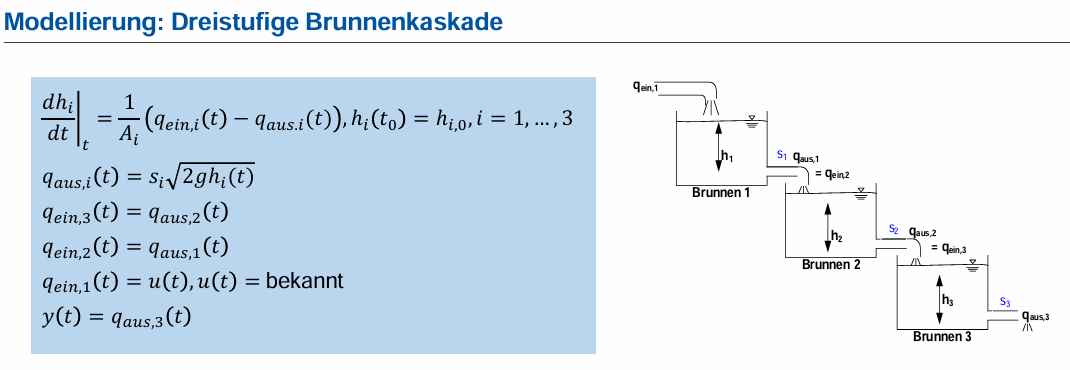
\includegraphics[width=0.8\textwidth]{figures/fountain_chain.png}
		\caption{Fountain Chain}
	\end{figure}
	{\tiny *Figure was taken from Simulationstechnik II, Prof. Alexander Mitsos, Ph.D.}
\end{frame}
	
\begin{frame}[fragile]
\frametitle{Software Tests: Case Study for v2.5 \\
	\small \color{rwth-blue} ODE: fountain chain}
	$r(0) = \frac{1}{p_2} \left( p_0 - p_3 \sqrt{2 p_1 x_0} \right)$
	
	$r(i) = \frac{1}{p_{2i+2}} \left( p_{2i+1} \sqrt{2 p_1 x_{i-1}} - p_{2i+3} \sqrt{2 p_1 x_i} \right), \quad i = 1, 2, ..., n-1$
	\begin{lstlisting}
		#pragma once
		#include "cppNum/differentialSystem/system.hpp"
		#include <cassert>
		
		template<typename T>
		la::vector_t<T> ds::system_t::G(const la::vector_t<T> &x, const la::vector_t<T> &p) {
		int n = x.size();
		assert(p.size() == 2*n + 2);
		assert(n >= 2);
		la::vector_t<T> r(n);
		r(0) = (1/p(2))*(p(0) - p(3)*sqrt(2*p(1)*x(0)));
		for(int i = 1; i < n; i++) {
			r(i) = (1/p(2*i + 2))*(p(2*i + 1)*sqrt(2*p(1)*x(i - 1)) - p(2*i + 3)*sqrt(2*p(1)*x(i)));
		}
		return r;
	}
	\end{lstlisting}
	For time measurements:
        \begin{itemize}
            \item Initial value of x: $[0, 0, ..., 0]$
			\item Parameters p: $[1, 9.81, 10, 1, ..., 10, 1]$, where $p(0)=1$ is input stream, $p(1)=9.81$ is acceleration of free fall, $p(2i)=10$ is area of fountain, $p(2i+1)=1$ is area of exit hole.
        \end{itemize}
\end{frame}
		
\begin{frame}[fragile]
\frametitle{Software Tests: Case Study for v2.5 \\
	\small \color{rwth-blue} ODE: linear ode}
	$\frac{d\mathbf{x}}{dt} = A \mathbf{x}$

	\begin{lstlisting}
		#pragma once
		#include "cppNum/differentialSystem/system.hpp"
		#include <cassert>
		
		template<typename T>
		la::vector_t<T> ds::system_t::G(const la::vector_t<T> &x, const la::vector_t<T> &p) {
		int n=x.size();
		assert(p.size()==n*n);
		la::vector_t<T> r=la::vector_t<T>::Zero(n);
		for(int i=0; i<n; i++)
			for(int j=0; j<n; j++)
			r(i)+=p(i*n+j)*x(j);
		return r;
		}
	\end{lstlisting}
	 For time measurements:
        \begin{itemize}
            \item initial value of x: $[1, 1, ..., 1]$
			\item Parameters p contain matrix $A=$
			{\tiny
			$\begin{bmatrix}
				-1 & -1 & 0 & 0 &... & 0\\
				1 & -1 & 0 & 0 &... & 0\\
				0 & 0 & -1-2/n & 0 & ... & 0\\
				... & ... & ... & ... & ... & ...\\
				0 & 0 & 0 & ... & 0 & -1-(n-1)/n 
			\end{bmatrix}$}
        \end{itemize}
\end{frame}
	
\begin{frame}
\frametitle{Software Tests v2.4: Run Time Difference \\
	\small \color{rwth-blue} Convex Polynomial and Cosh Function}
	\begin{figure}
		\centering
		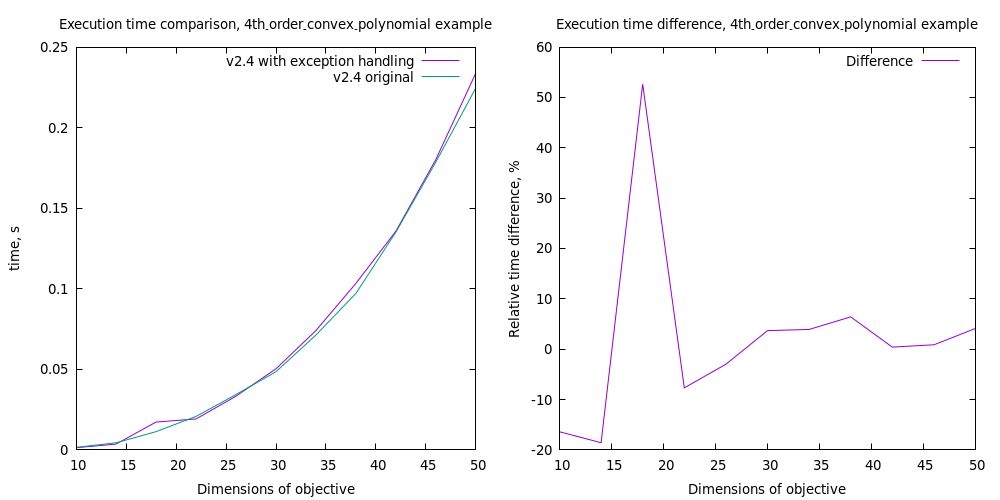
\includegraphics[width=0.65\textwidth]{figures/2.4_4th_order_convex_polynomial.png}
		\vspace{0.3cm}
		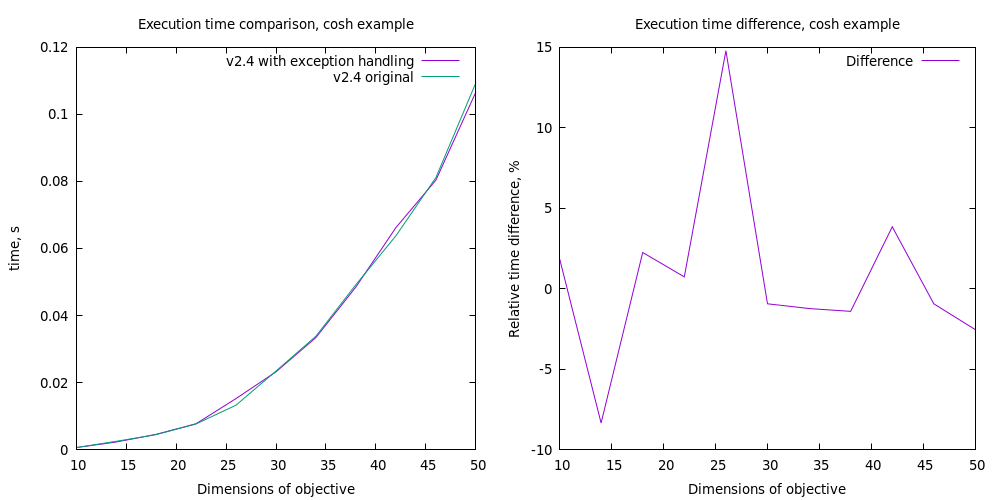
\includegraphics[width=0.65\textwidth]{figures/2.4_cosh.png}
	\end{figure}
\end{frame}
	
\begin{frame}
\frametitle{Software Tests v2.5: Run Time Difference \\
	\small \color{rwth-blue} Fountain Chain and Linear ODE}
	\begin{figure}
		\centering
		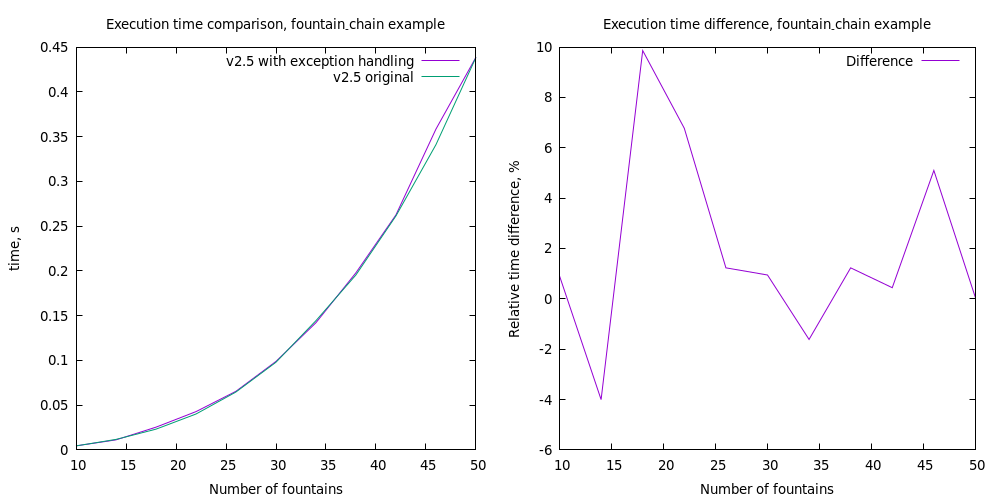
\includegraphics[width=0.65\textwidth]{figures/2.5_fountain_chain.png}
		\vspace{0.3cm}
		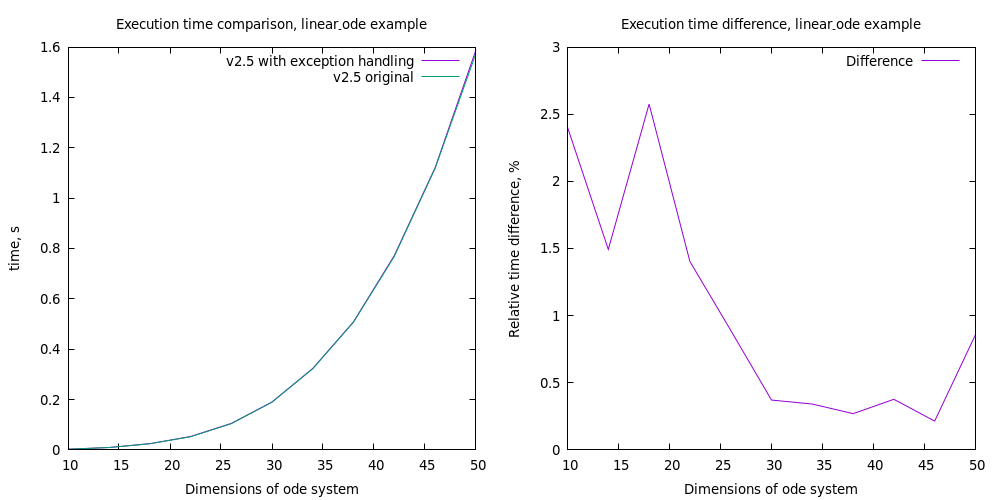
\includegraphics[width=0.65\textwidth]{figures/2.5_linear_ode.png}
	\end{figure}
\end{frame}
	
\begin{frame}
\frametitle{Software Tests: Run Time Difference \\
	\small \color{rwth-blue} Conclusion}
	\begin{itemize}
		\item Differences between the versions with and without exception handling under different problem sizes:
		\begin{itemize}
			\item For small problems, the difference between versions varies between runs because small problems are particularly affected by fluctuations in processor performance (if the processor is busy with operating system tasks).
			\item The overall difference is small because the resources used for exception handling in the program are very minimal and almost negligible. 
			\item Most of the resources are utilized for performing algorithmic differentiation and solving the linear algebraic system at each step.
		\end{itemize}
	\end{itemize}
\end{frame}
			
\section{Project Management}
\begin{frame}
\frametitle{Project Management \\
	\small \color{rwth-blue} Task}
	\begin{itemize}	
			\item \textbf{1.Self-study course:}
				\begin{itemize}
					\item Discuss problems in group in Discord.
					\item Read source code.
				\end{itemize}
			\item \textbf{2.Extend cppNum with exception handling:}
				\begin{itemize}
					\item Classification of Exceptions
					\item Create exception classes
					\item Add exception classes with try-catch to source code
				\end{itemize}
			\item \textbf{3.Design scalable case studies:}
				\begin{itemize}
				\item Implent new cases
				\item Add timing and plotting method
				\item Visualization
				\item Test and Debug
				\end{itemize}
			\item \textbf{4.Run time difference Analysis:}
			\item \textbf{5.Presentation:}
				\begin{itemize}
				\item Analysis (user requirements , use case)
				\item Source code and design
				\item Project management and live-demo(test)
				\item Case study(example) and run time analysis
				\end{itemize}
			\item *The following page of the PDF outlines the responsibilities of each person.
	\end{itemize}
\end{frame}
	
\begin{frame}
\frametitle{Project Management \\
	\small \color{rwth-blue} Gantt Chart}
	
	\begin{center}
		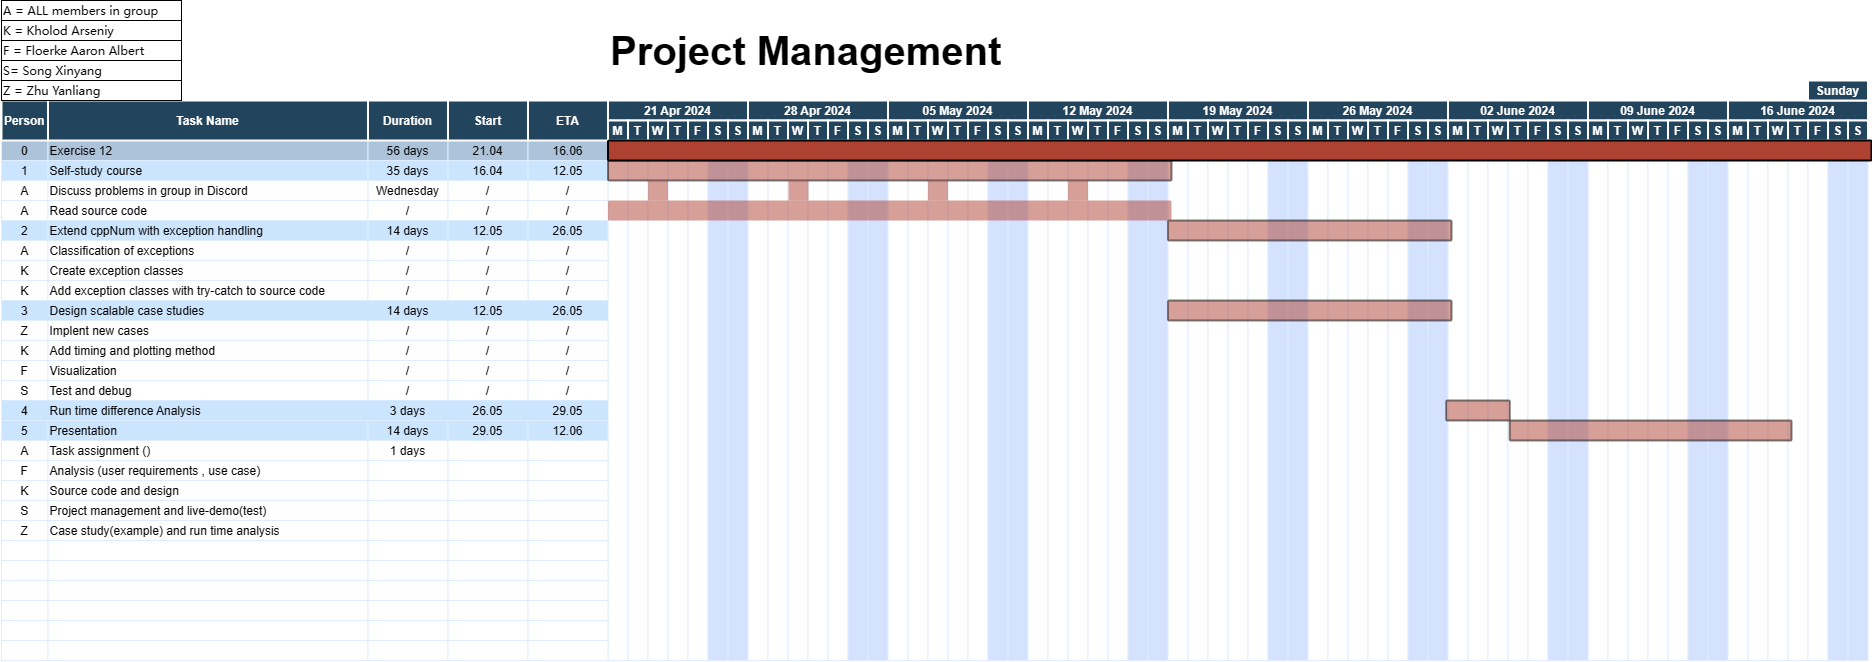
\includegraphics[width=\textwidth]{figures/project management.png}
	\end{center}
\end{frame}

\begin{frame}
\frametitle{Project Management \\
	\small \color{rwth-blue} Task Assignment}
	
	\begin{flushleft}
		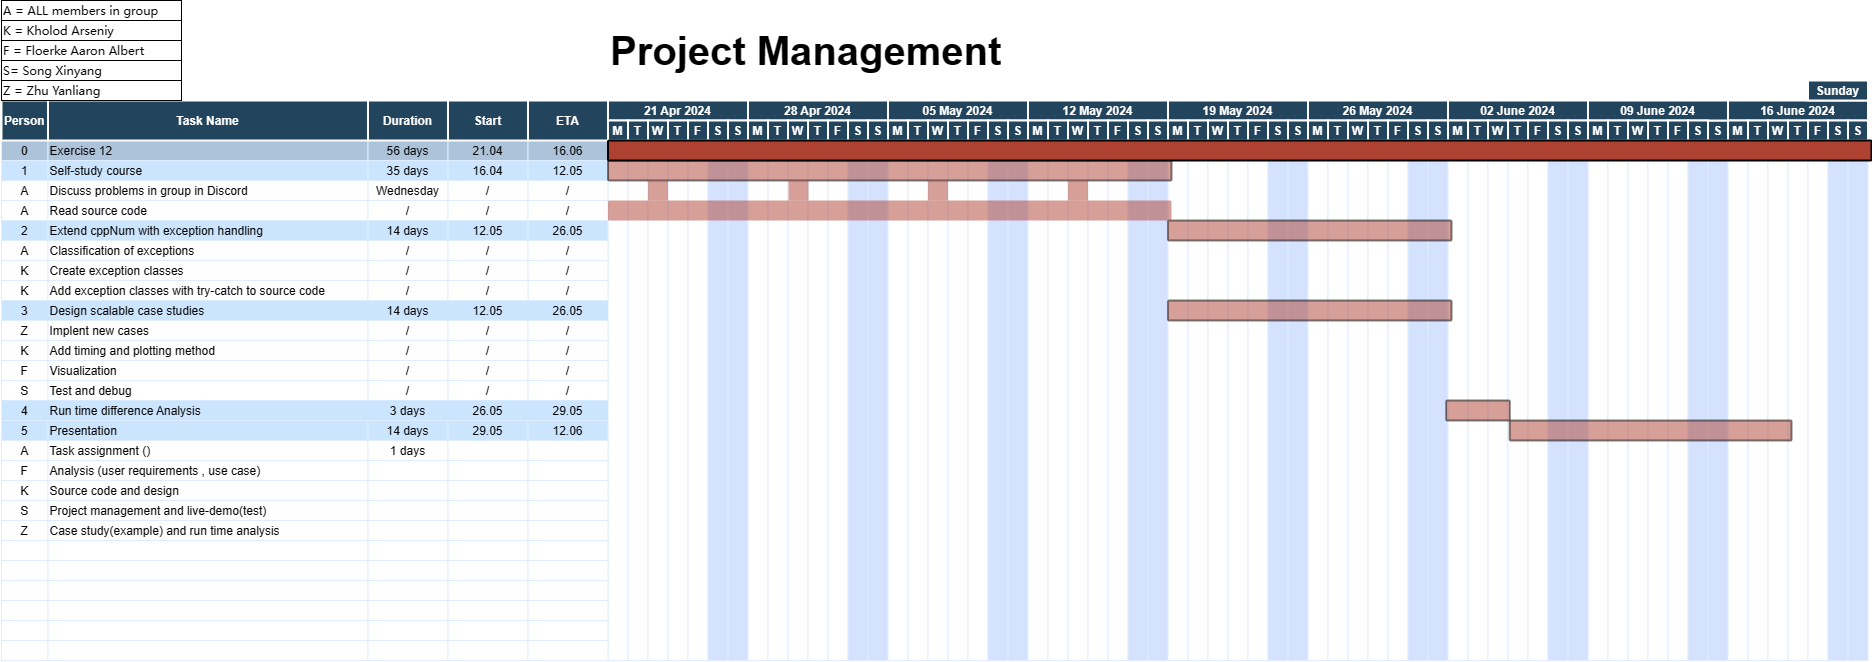
\includegraphics[height=\textheight,keepaspectratio]{figures/project management.png}
	\end{flushleft}
\end{frame}
	
\section{Live Demo}

\begin{frame}[fragile]
\frametitle{Live Demo v2.4 \\
	\small \color{rwth-blue} Run in Xubuntu}
	Use function: $y=\frac{1}{2}x_1^2+\frac{1}{2}x_2^2+x_1 x_2$ for minimization with Newton method (cppNum v2.4).

	Hessian matrix: $\partial^2y=\begin{bmatrix}1&&1\\1&&1\end{bmatrix}$ is singular, so minimization with Newton method is not applicable.
	
	\textbf{Show live demo}:
	\begin{itemize}
        	\item 1.Build executable: make
        	\item 2.Execute: ./main.exe
	\end{itemize}
	Output of the live demo:
	\begin{lstlisting}[language=bash]
		Exception was caught in la::lu_solver_t::run, throw it further.
		Exception was caught in as::newton_solver_t::run, throw it further.
		std:exception was caught in co::newton_minimizer_t::run with following message:
		Matrix is singular, applying LU algorithm for solving a linear system is not possible.
		co::newton_minimizer_t::run returns an initial value of x. Check the correctness of the input.
	\end{lstlisting}
	In the output, one can observe a stack trace and a message describing the exception. 
\end{frame}



\section{Summary and Conclusion}

\begin{frame}
\frametitle{Summary and Conclusion}
	\begin{itemize}
		\item Analysis was conducted to determine essential system requirements.
		\item Exception handling mechanism was added to cppNum v2.4 and v2.5:
		\begin{itemize}
			\item Exceptions from Eigen and AD were handled by wrapping connection points in try blocks.
			\item cppNum exception classes were created and used to throw exceptions in case of bad input.
		\end{itemize}
		\item New classes were documented with Doxygen.
		\item Four scalable use cases were designed (two for v2.4 and two for v2.5).
		\item Runtime experiments were conducted to demonstrate minimal performance degradation.
		\item Project management was handled using a Gantt chart.
	\end{itemize}
\end{frame}

\end{document}
